\section{Results and Evaluation of Methods}\label{section:statistics_results}

To evaluate the effectiveness of the process of sequentially minimising the probability bounds on the error of the sample estimated stratified mean, we need a little development of those algorithms before proceeding to give details on the process of testing them in the context of synthetic data.

Particularly it is necessary to consider the way in which the concentration inequality of the previous section (Theorem \ref{thm:SEBM_bound}) should be iteratively minimised; and this process is expounded as Algorithm \ref{alg2}.
Additionally it is necessary to give some explication to how the concentration inequalities derived from EBBs (per Theorem \ref{triangle_theorem2}) should be sequentially minimised; and this process is expounded as Algorithm \ref{alg3}.

In this section, these different schemes of sampling in the context of Stratified sampling are compared primarily in the context of Beta-distributed data - but also in a more specific Bernoulli-uniform data set, where they are also compared against Neyman sampling, and simple random sampling; all this comparison occurs in Section \ref{sec:application}.

Following this section we also consider the effectiveness of different methods of sampling specifically to approximate the Shapley Value.

\subsection{Sequential Sampling Using the Stratified Empirical Berstein Method} \label{sec:SEBMalgorithm}
In the previous section \ref{section:SEBB}, we developed a concentration inequality to bound the error of the sampling mean estimate in stratified random sampling, called the SEBB - as per Theorem \ref{thm:SEBM_bound}.
The process of selecting additional samples to minimise this probability bound on the error is introduced in this section. And we call it the \textit{stratified empirical Bernstein method} (SEBM).

The fundamental principle of the SEBM, is that it is an online method of choosing additional samples, and to do this it scans through all the possible strata from which it can take an additional sample, and as it does so it calculates the possible reduction in the SEBB bound that would be achieved if an additional sample were taken from the respective strata.
The strata which would result in the most reduction of the SEBB bound is then recommended for additional sampling.
The pseudo-code for this process of sampling, is given as Algorithm \ref{alg2}.



Specifically, Algorithm \ref{alg2} is a repetitive process involving a scan through the possible strata and then the selection of one stratum to sample from to minimize the SEBB under mild assumptions.
The process of scanning involves calculating the confidence bound width (SEBB) that would result if an additional sample were to be taken from that stratum without changing its sample variance (line numbers 5-17 in Algorithm~\ref{alg2}).
The stratum that yields the smallest confidence bound width in the context of an additional sample is then selected (line 18-21) and sampled (line 24), the sample variance of that stratum is updated (line 26); 
this process repeats until the maximum sample budget is reached (per the outer loop, line 1).
In this way the process attempts to iteratively minimize the SEBB in expectation with each additional sample taken; and hence lead to potentially greater accuracy in stratified sampling as a result.

The primary assumption that exists in this method's selection calculus is that it assumes that the sample variance of the strata would likely remain unchanged for the taking of the additional sample from any strata.
While this technically isn't true, the unbiased sample variance is intuitively be expected to be almost as likely to increase as it is likely to decrease from the taking of an additional sample.
Plus developing an even more complicated probability bound that explicitly takes account of the likely change in error of the stratified mean estimate due to the expected change in the sample variance is beyond the scope of our investigation.

This SEBM method (Algorithm \ref{alg2}) requires the sample variances of all the strata to be calculated. And accordingly, Algorithm \ref{alg2} must be initialized with at least two samples from each stratum so that sample variance can be calculated for it to be able to function.
And this is a standard requirement of the many reinforcement learning algorithms that use variance in their sampling policies.

We also note that Algorithm \ref{alg2} describes a process specific to the sampling without replacement of all strata, and involves the calculation of the SEBB with the tightest possible use cases of Lemmas \ref{martingale0} and~\ref{martingale1}.
In particular, for any stratum $i$ that is sampled without replacement, any specific bound with an associated $\Omega_{m_i}^{n_i}$ and $\Psi_{m_i}^{n_i}$ may be substituted for $\bar{\Omega}_{m_i}^{n_i}$ and $\bar{\Psi}_{m_i}^{n_i}$ to potentially tighten the bound, and this corresponds to choice of Lemma~\ref{martingale0} or Lemma~\ref{martingale1} in the bound's derivation. 
Since the SEBB is a composition of such bounds with such choices throughout, there is a structure of valid pairs of substitutions $\Omega,\Psi$ for $\bar{\Omega},\bar{\Psi}$ in the optimal calculation of the SEBB, which is shown in the steps 8-15 of Algorithm \ref{alg2}.
The equivalent algorithm for sampling with replacement simply is the same algorithm altered by replacing all use of $\bar{\Omega},\bar{\Psi}$ with $\Omega,\Psi$ respectively.

\begin{algorithm}
\caption{Stratified Empirical Bernstein Method (SEBM) with replacement}
\label{alg2}
\begin{algorithmic}[1]
    \REQUIRE probability $p$, strata number $N$, stratum sizes $n_i$, initial sample numbers $m_i$, initial stratum sample variances $\doublehat{\sigma}_i^2$, weights $\tau_i$, widths $D_i$, maximum sample budget $B$
    \WHILE{$\sum_i{m_i}<B$}
        \STATE $beststrata \leftarrow -1$
        \STATE $lowestbound \leftarrow \infty$
    	\FOR{$k=0$ to $N$}
    	    \STATE $m_k \leftarrow m_k + 1$
        	\STATE $a \leftarrow [0,0]$, $b \leftarrow [0,0]$, $c \leftarrow [0,0]$, $d \leftarrow [0,0]$
        	\FOR{$i=0$ to $N$}
        		\STATE $a_0 \leftarrow a_0 + \log(6N/p)D_i^2\bar{\Psi}_{m_i}^{n_i}\min(\bar{\Omega}_{m_i}^{n_i},\Omega_{m_i}^{n_i})\tau^2$
        		\STATE $a_1 \leftarrow a_1 + \log(6N/p)D_i^2\Psi_{m_i}^{n_i}\min(\bar{\Omega}_{m_i}^{n_i},\Omega_{m_i}^{n_i})\tau^2$
        		\STATE $b_0 \leftarrow \max(b_0,\log(3/p)D_i^2\bar{\Psi}_{m_i}^{n_i}\min(\bar{\Psi}_{m_i}^{n_i},\Psi_{m_i}^{n_i})\tau^2)$
        		\STATE $b_1 \leftarrow \max(b_1,\log(3/p)D_i^2\Psi_{m_i}^{n_i}\min(\bar{\Psi}_{m_i}^{n_i},\Psi_{m_i}^{n_i})\tau^2)$
        		\STATE $c_0 \leftarrow c_0 + 2\bar{\Psi}_{m_i}^{n_i}((m_i-1)\doublehat{\sigma}_i^2/m_i)\tau^2$
        		\STATE $c_1 \leftarrow c_1 + 2\Psi_{m_i}^{n_i}((m_i-1)\doublehat{\sigma}_i^2/m_i)\tau^2$
        		\STATE $d_0 \leftarrow d_0 + \frac{4}{17}D_i^2\bar{\Omega}_{m_i}^{n_i}\tau^2$
        		\STATE $d_1 \leftarrow d_1 + \frac{4}{17}D_i^2\Omega_{m_i}^{n_i}\tau^2$
        	\ENDFOR
        	\STATE $boundwidth \leftarrow \sqrt{\log(6/p)\min_j(d_j + (\sqrt{c_j + a_j + b_j} + \sqrt{b_j})^2)}$
    	    \IF{$boundwidth < lowestbound$}
    	        \STATE $beststrata \leftarrow k$
    	        \STATE $lowestbound \leftarrow boundwidth$
    	    \ENDIF
    	    \STATE $m_k \leftarrow m_k - 1$
    	\ENDFOR
    	\STATE take an extra sample from strata: $beststrata$
	    \STATE $m_{beststrata} \leftarrow m_{beststrata} + 1$
    	\STATE recalculate $\doublehat{\sigma}_{beststrata}^2$
    \ENDWHILE
\end{algorithmic}
\end{algorithm}


In the next part we give an algorithm and pseudo-code corresponding to the minimising of error bounds for stratified sampling created by EBBs, via Theorem \ref{triangle_theorem2}.



\subsection{Sequential Sampling Using Unionised EBBs} \label{sec:EBBalgorithm}

In the section \ref{section:old_statistics} of this chapter we considered different possible EBBs as a means of creating bounds for the error in stratified sampling. And that choosing additional samples to minimise these bounds function as a method of choosing samples in the context of stratified sampling.
This method is made clear in pseudocode in algorithm \ref{alg3}.


\begin{algorithm}
\caption{Stratified Error bound reduction by unionised EBBs - by Theorem \ref{triangle_theorem2}}
\label{alg3}
\begin{algorithmic}[1]
    \REQUIRE probability $t$, strata number $N$, stratum sizes $n_i$, initial sample numbers $m_i$, initial stratum sample variances $\doublehat{\sigma}_i^2$, weights $\tau_i$, widths $D_i$, maximum sample budget $B$.
    We assume an Empirical Bernstein Bound $Z$ as per the following form:
$\quad \p(\hat{\mu}_i-\mu_i \ge Z(m_i,D_i,\hat{\sigma}^2_i,t)) \le t $
    \WHILE{$\sum_i{m_i}<B$}
        \STATE $beststrata \leftarrow -1$
        \STATE $bestimprovement \leftarrow 0$
    	\FOR{$k=0$ to $N$}
    		\STATE $improvement \leftarrow \frac{n_i}{\sum_kn_k}\left(Z(m_i,D_i,\hat{\sigma}^2_i,t) - Z(m_i+1,D_i,\hat{\sigma}^2_i,t)\right)$
    	    \IF{$improvement > bestimprovement$}
    	        \STATE $beststrata \leftarrow k$
    	        \STATE $bestimprovement \leftarrow improvement$
    	    \ENDIF
    	\ENDFOR
    	\STATE take an extra sample from strata: $beststrata$
	    \STATE $m_{beststrata} \leftarrow m_{beststrata} + 1$
    	\STATE recalculate $\doublehat{\sigma}_{beststrata}^2$
    \ENDWHILE
\end{algorithmic}
\end{algorithm}




%\begin{theorem}\label{triangle_theorem1}
%If we have $m$ strata of sizes $N_i$. If we have taken $n_i$ samples $X_{i,1},X_{i,2},\dots,X_{i,n_i}$ from each stratum, resulting in a stratum sample mean $\hat{\mu}_i = \frac{1}{n_i}\sum_{j=1}^{n_i}X_{i,j}$ and stratum sample variance $\hat{\sigma}_i^2=\frac{1}{n_i}\sum_{j=1}^{n_i}(X_{i,j}-\hat{\mu}_i)^2 $.
%If the error in the sample mean of a stratum is bounded by an Empirical Bernstein Bound:
%$\quad \p(\hat{\mu}_i-\mu_i \ge Z(n_i,D_i,\hat{\sigma}^2_i,t)) \le t $\\
%Then the error in our stratified estimation is probability bounded:
%$$ \p\left(\hat{\mu}-\mu \ge \sum_{i=1}^m\frac{N_i}{\sum_kN_k} Z(n_i,D_i,\hat{\sigma}^2_i,t/m)\right)\le t $$
%\end{theorem}






In the next Section~\ref{sec:application} we evaluate the performance of SEBM with other methods in the context of synthetic data.


\pagebreak
\section{Numerical Evaluation}\label{sec:application}

In this section assess the value of SEBM as an online method of sampling from stratified data.
First we outline the benchmark algorithms used to evaluate our method's performance.
Then in Section~\ref{ssec:SyntheticDists}
we describe two synthetic data sets and report the distribution of errors under our method and the benchmarks.
Following this, in Section~\ref{sec:shapley}, we evaluate our method in an example application --- that of calculating the Shapley value of a cooperative game.
Discussion and analysis of all the numerical results is left to Section~\ref{sec:discussion}.



\subsection{Benchmarks algorithms}
In the numerical evaluations, we compare the following sampling methods:
\begin{itemize}
\item 
\textsc{SEBM} (Stratified empirical Bernstein method, without replacement):
our SEBM method (per Algorithm \ref{alg2}) of iteratively choosing samples from strata to minimize the SEBB, given in Equation~\eqref{big_equation}. 
An initial sample of two data points from each strata is used to initialize the sample variances of each, with additional samples made to maximally minimize the inequality at each step. All samples are drawn \textit{without} replacement.
\item 
\textsc{SEBM-W} (Stratified empirical Bernstein method with replacement): 
as above, with the exception that all samples are drawn \textit{with} replacement, and consequently the inequality does not utilize the martingale inequality given in Lemma~\ref{martingale0}.
\item 
\textsc{Sim} (Simple random sampling, without replacement): simple random sampling from the population irrespective of strata \textit{without} replacement.
\item 
\textsc{Sim-W} (Simple random sampling with replacement): 
simple random sampling from the population irrespective of strata \textit{with} replacement.
\item \textsc{Ney} (Neyman sampling, without replacement): the method of maximally choosing samples \textit{without} replacement from strata proportional to the strata variance.
\item \textsc{Ney-W} (Neyman sampling with replacement): the method of choosing samples \textit{with} replacement proportional to the strata variance.
\item \textsc{SEBM*} (Stratified empirical Bernstein method with variance assistance): the method of iteratively choosing samples \textit{without} replacement from strata to minimize Equation~\eqref{eq1}, utilizing martingale Lemma~\ref{martingale0}.
\end{itemize}
Note that the last three methods (\textsc{Ney},\textsc{Ney-W} and SEBM*) assume and utilize prior perfect knowledge of the variance of each of the strata, and that for methods SEBM, SEBM-W and SEBM* (which use Equations~\eqref{big_equation} and~\eqref{eq1}) we selected for minimising a 50\% confidence interval (i.e. constant $p=0.5$ and $t=0.5$).

Also note that these methods provide comparisons of different algorithm factors, such as the dynamics of sampling: with and without replacement; with stratification and without; between our method and Neyman sampling, and; with and without perfect knowledge of stratum variances. 
For these methods, we consider the effectiveness against beta distributed data and for a case of uniform-and-Bernoulli data.
% Detailed analysis of the results is left to Section~\ref{sec:discussion}.

\subsection{Synthetic Data}
\label{ssec:SyntheticDists}
The first way we demonstrate the efficacy of our method is to generate sets of synthetic data, and then numerically examine the distribution of errors generated by different methods of choosing finite sequences of samples.
In this section, we described the two types of synthetic data sets used in this evaluation, namely: 
(i) beta distributed stratum data, which are intended reflect real-world data, and 
(ii) a particular form of uniform and Bernoulli distributed stratum data, in which our sampling method (SEBM) performs poorly.

\subsubsection{Beta-Distributed Data}
The first pool of synthetic data % sets are intended to be representative of potential real-world data.
% These sets 
have between 5 and 21 strata, with the number of strata drawn with uniform probability, 
and each strata sub-population has sizes ranging from 10 to 201, also drawn uniformly.
The data values in each strata are drawn from beta distributions, with classic probability density function:
$$\phi(x)_{\{\alpha,\beta\}}
=\frac{\Gamma(\alpha+\beta)}{\Gamma(\alpha)\Gamma(\beta)}     
    x^{\alpha-1}(1-x)^{\beta-1} $$
with $\alpha$ and $\beta$ parameters drawn uniformly between 0 and 4 for each stratum, and $\Gamma$ is gamma function.






\begin{figure}
    \centering
    \resizebox{0.48\textwidth}{!}{
    \begin{tikzpicture}[]
    		\begin{axis}[
			title={10N sample budget},
    		boxplot/draw direction=y,
    		x axis line style={opacity=0},
    		y axis line style={opacity=10},
    		tick style={opacity=0},
    		%xticklabel style={opacity=0},
    		axis x line*=bottom,
    		axis y line=left,
    		enlarge y limits,
    		ymajorgrids,
    		minor y tick num=1,
    		yminorgrids,
    		xtick={1,2,3,4,5,6,7,8,9,10},
    		xticklabels={
    			\STAB{\rotatebox[origin=c]{90}{\textsc{SECM-W}}}, 
    			\STAB{\rotatebox[origin=c]{90}{\textsc{SEBM*-W}}},
    			\STAB{\rotatebox[origin=c]{90}{\textsc{SEBM-W}}},
    			\STAB{\rotatebox[origin=c]{90}{\textsc{Ney-W}}},
    			\STAB{\rotatebox[origin=c]{90}{\textsc{Hoeffding}}},
    			\STAB{\rotatebox[origin=c]{90}{\textsc{Audibert}}},
    			\STAB{\rotatebox[origin=c]{90}{\textsc{Maurer}}},
    			\STAB{\rotatebox[origin=c]{90}{\textsc{EEBB}}},
    			\STAB{\rotatebox[origin=c]{90}{\textsc{Random}}},
    			\STAB{\rotatebox[origin=c]{90}{\textsc{Simple-W}}},
    			},
    		]
% -- SECM-W
\addplot [boxplot prepared={lower whisker=0.00203711817479,lower quartile=0.00590714931702,median=0.0126957428186,upper quartile=0.0216502921928,upper whisker=0.0339253899173 }] coordinates {};
% -- SEBM*-W
\addplot [boxplot prepared={lower whisker=0.00195105293753,lower quartile=0.00579327577325,median=0.0119512053277,upper quartile=0.0209721064657,upper whisker=0.0319103845748 }] coordinates {};
% -- SEBM-W
\addplot [boxplot prepared={lower whisker=0.00214321028201,lower quartile=0.00601160251813,median=0.0124363175098,upper quartile=0.0212232972856,upper whisker=0.033180153486 }] coordinates {};
% -- Ney-W
\addplot [boxplot prepared={lower whisker=0.00205089432254,lower quartile=0.00572207687956,median=0.0116932754283,upper quartile=0.0207321361345,upper whisker=0.0316086258607 }] coordinates {};
% -- Hoeffding
\addplot [boxplot prepared={lower whisker=0.00204855603277,lower quartile=0.00590792248556,median=0.0123188066961,upper quartile=0.0215342168159,upper whisker=0.0339059739931 }] coordinates {};
% -- Audibert
\addplot [boxplot prepared={lower whisker=0.00197716643965,lower quartile=0.00580743977862,median=0.0126351819423,upper quartile=0.0215678269509,upper whisker=0.0346573104751 }] coordinates {};
% -- Maurer
\addplot [boxplot prepared={lower whisker=0.00204915265935,lower quartile=0.00588924949337,median=0.0125159072736,upper quartile=0.0223133553934,upper whisker=0.0347450423664 }] coordinates {};
% -- EEBB
\addplot [boxplot prepared={lower whisker=0.00208350815087,lower quartile=0.00597848454177,median=0.0128126936436,upper quartile=0.0219542739196,upper whisker=0.0336397274961 }] coordinates {};
% -- Random
\addplot [boxplot prepared={lower whisker=0.00248342203622,lower quartile=0.00688208349805,median=0.0144683105789,upper quartile=0.0250518713876,upper whisker=0.0383944963878 }] coordinates {};
% -- Simple-W
\addplot [boxplot prepared={lower whisker=0.0031217187683,lower quartile=0.00863729366985,median=0.0187203946103,upper quartile=0.032091144832,upper whisker=0.0482844458999 }] coordinates {};
				\end{axis}
			\end{tikzpicture}}%
\hfill\resizebox{0.48\textwidth}{!}{\begin{tikzpicture}[]
    		\begin{axis}[
			title={50N sample budget},
    		boxplot/draw direction=y,
    		x axis line style={opacity=0},
    		y axis line style={opacity=10},
    		tick style={opacity=0},
    		%xticklabel style={opacity=0},
    		axis x line*=bottom,
    		axis y line=left,
    		enlarge y limits,
    		ymajorgrids,
    		minor y tick num=1,
    		yminorgrids,
    		xtick={1,2,3,4,5,6,7,8,9,10},
    		xticklabels={
    			\STAB{\rotatebox[origin=c]{90}{\textsc{SECM-W}}}, 
    			\STAB{\rotatebox[origin=c]{90}{\textsc{SEBM*-W}}},
    			\STAB{\rotatebox[origin=c]{90}{\textsc{SEBM-W}}},
    			\STAB{\rotatebox[origin=c]{90}{\textsc{Ney-W}}},
    			\STAB{\rotatebox[origin=c]{90}{\textsc{Hoeffding}}},
    			\STAB{\rotatebox[origin=c]{90}{\textsc{Audibert}}},
    			\STAB{\rotatebox[origin=c]{90}{\textsc{Maurer}}},
    			\STAB{\rotatebox[origin=c]{90}{\textsc{EEBB}}},
    			\STAB{\rotatebox[origin=c]{90}{\textsc{Random}}},
    			\STAB{\rotatebox[origin=c]{90}{\textsc{Simple-W}}},
    			},
    		]
% -- SECM-W
\addplot [boxplot prepared={lower whisker=0.000873614811035,lower quartile=0.00256230207769,median=0.00549196590068,upper quartile=0.00947419398793,upper whisker=0.0146663481198 }] coordinates {};
% -- SEBM*-W
\addplot [boxplot prepared={lower whisker=0.000910092361617,lower quartile=0.00250624851109,median=0.00542288378302,upper quartile=0.00938662860078,upper whisker=0.0145620218616 }] coordinates {};
% -- SEBM-W
\addplot [boxplot prepared={lower whisker=0.000951411349914,lower quartile=0.00260844954482,median=0.00549365633573,upper quartile=0.00959589925114,upper whisker=0.0149751426419 }] coordinates {};
% -- Ney-W
\addplot [boxplot prepared={lower whisker=0.000887479040566,lower quartile=0.00247214781011,median=0.00542124962027,upper quartile=0.00939389449743,upper whisker=0.0141671187264 }] coordinates {};
% -- Hoeffding
\addplot [boxplot prepared={lower whisker=0.000966512003819,lower quartile=0.00267673077629,median=0.00555753121815,upper quartile=0.00956064483231,upper whisker=0.0145705059888 }] coordinates {};
% -- Audibert
\addplot [boxplot prepared={lower whisker=0.000939560847084,lower quartile=0.00256020151103,median=0.00546386150453,upper quartile=0.00973905959264,upper whisker=0.0151597017036 }] coordinates {};
% -- Maurer
\addplot [boxplot prepared={lower whisker=0.000923515948706,lower quartile=0.00260380941632,median=0.00561513487346,upper quartile=0.00984308947158,upper whisker=0.0145168898968 }] coordinates {};
% -- EEBB
\addplot [boxplot prepared={lower whisker=0.000880018992369,lower quartile=0.00265879716358,median=0.00558553639166,upper quartile=0.00957392266325,upper whisker=0.0150260400173 }] coordinates {};
% -- Random
\addplot [boxplot prepared={lower whisker=0.00100378500126,lower quartile=0.00292551330324,median=0.00614395616333,upper quartile=0.0106715749674,upper whisker=0.0161770606241 }] coordinates {};
% -- Simple-W
\addplot [boxplot prepared={lower whisker=0.00132457947878,lower quartile=0.00382970607309,median=0.00806642336181,upper quartile=0.0139247953938,upper whisker=0.0218688980015 }] coordinates {};
				\end{axis}
			\end{tikzpicture}}
\\
\resizebox{0.48\textwidth}{!}{\begin{tikzpicture}[]
    		\begin{axis}[
			title={100N sample budget},
    		boxplot/draw direction=y,
    		x axis line style={opacity=0},
    		y axis line style={opacity=10},
    		tick style={opacity=0},
    		%xticklabel style={opacity=0},
    		axis x line*=bottom,
    		axis y line=left,
    		enlarge y limits,
    		ymajorgrids,
    		minor y tick num=1,
    		yminorgrids,
    		xtick={1,2,3,4,5,6,7,8,9,10},
    		xticklabels={
    			\STAB{\rotatebox[origin=c]{90}{\textsc{SECM-W}}}, 
    			\STAB{\rotatebox[origin=c]{90}{\textsc{SEBM*-W}}},
    			\STAB{\rotatebox[origin=c]{90}{\textsc{SEBM-W}}},
    			\STAB{\rotatebox[origin=c]{90}{\textsc{Ney-W}}},
    			\STAB{\rotatebox[origin=c]{90}{\textsc{Hoeffding}}},
    			\STAB{\rotatebox[origin=c]{90}{\textsc{Audibert}}},
    			\STAB{\rotatebox[origin=c]{90}{\textsc{Maurer}}},
    			\STAB{\rotatebox[origin=c]{90}{\textsc{EEBB}}},
    			\STAB{\rotatebox[origin=c]{90}{\textsc{Random}}},
    			\STAB{\rotatebox[origin=c]{90}{\textsc{Simple-W}}},
    			},
    		]
% -- SECM-W
\addplot [boxplot prepared={lower whisker=0.000636850883585,lower quartile=0.001758421023,median=0.00380445489544,upper quartile=0.00670922210984,upper whisker=0.0102776964 }] coordinates {};
% -- SEBM*-W
\addplot [boxplot prepared={lower whisker=0.000632386155924,lower quartile=0.00176154976274,median=0.00379949013741,upper quartile=0.00671829236954,upper whisker=0.0103315144235 }] coordinates {};
% -- SEBM-W
\addplot [boxplot prepared={lower whisker=0.000680754753892,lower quartile=0.00185837687059,median=0.00386209609049,upper quartile=0.00658796718008,upper whisker=0.00995840759784 }] coordinates {};
% -- Ney-W
\addplot [boxplot prepared={lower whisker=0.000657938325888,lower quartile=0.0017444987029,median=0.0037713834643,upper quartile=0.00656878044395,upper whisker=0.0101006080514 }] coordinates {};
% -- Hoeffding
\addplot [boxplot prepared={lower whisker=0.000649029201759,lower quartile=0.0018278581662,median=0.00385518249136,upper quartile=0.00664697484699,upper whisker=0.0103246816298 }] coordinates {};
% -- Audibert
\addplot [boxplot prepared={lower whisker=0.000619859954485,lower quartile=0.00180976489989,median=0.00396390201518,upper quartile=0.00688077381745,upper whisker=0.0105260370656 }] coordinates {};
% -- Maurer
\addplot [boxplot prepared={lower whisker=0.000680406278875,lower quartile=0.00193778416988,median=0.00401502678431,upper quartile=0.00701666928955,upper whisker=0.0103290413186 }] coordinates {};
% -- EEBB
\addplot [boxplot prepared={lower whisker=0.000594144270816,lower quartile=0.00177108325136,median=0.0039677038012,upper quartile=0.00689698780572,upper whisker=0.0104024014189 }] coordinates {};
% -- Random
\addplot [boxplot prepared={lower whisker=0.00074150837092,lower quartile=0.00207314536165,median=0.00436685107489,upper quartile=0.00747350995688,upper whisker=0.0113332527557 }] coordinates {};
% -- Simple-W
\addplot [boxplot prepared={lower whisker=0.00105915507933,lower quartile=0.00270478575028,median=0.00575982393074,upper quartile=0.0100186063529,upper whisker=0.0154659123488 }] coordinates {};
				\end{axis}
			\end{tikzpicture}}%
\hfill\resizebox{0.48\textwidth}{!}{\begin{tikzpicture}[]
    		\begin{axis}[
			title={150N sample budget},
    		boxplot/draw direction=y,
    		x axis line style={opacity=0},
    		y axis line style={opacity=10},
    		tick style={opacity=0},
    		%xticklabel style={opacity=0},
    		axis x line*=bottom,
    		axis y line=left,
    		enlarge y limits,
    		ymajorgrids,
    		minor y tick num=1,
    		yminorgrids,
    		xtick={1,2,3,4,5,6,7,8,9,10},
    		xticklabels={
    			\STAB{\rotatebox[origin=c]{90}{\textsc{SECM-W}}}, 
    			\STAB{\rotatebox[origin=c]{90}{\textsc{SEBM*-W}}},
    			\STAB{\rotatebox[origin=c]{90}{\textsc{SEBM-W}}},
    			\STAB{\rotatebox[origin=c]{90}{\textsc{Ney-W}}},
    			\STAB{\rotatebox[origin=c]{90}{\textsc{Hoeffding}}},
    			\STAB{\rotatebox[origin=c]{90}{\textsc{Audibert}}},
    			\STAB{\rotatebox[origin=c]{90}{\textsc{Maurer}}},
    			\STAB{\rotatebox[origin=c]{90}{\textsc{EEBB}}},
    			\STAB{\rotatebox[origin=c]{90}{\textsc{Random}}},
    			\STAB{\rotatebox[origin=c]{90}{\textsc{Simple-W}}},
    			},
    		]
% -- SECM-W
\addplot [boxplot prepared={lower whisker=0.000695554212997,lower quartile=0.00198255695079,median=0.00414898985951,upper quartile=0.00736703210091,upper whisker=0.0112916958641 }] coordinates {};
% -- SEBM*-W
\addplot [boxplot prepared={lower whisker=0.000725448205883,lower quartile=0.00198498542637,median=0.0041411778437,upper quartile=0.00732886195779,upper whisker=0.0110886274658 }] coordinates {};
% -- SEBM-W
\addplot [boxplot prepared={lower whisker=0.000708781340772,lower quartile=0.00198244734804,median=0.00425386140966,upper quartile=0.00732022901583,upper whisker=0.0110975018936 }] coordinates {};
% -- Ney-W
\addplot [boxplot prepared={lower whisker=0.000680202868957,lower quartile=0.00196278935024,median=0.00412493148609,upper quartile=0.00709093376861,upper whisker=0.0107408704413 }] coordinates {};
% -- Hoeffding
\addplot [boxplot prepared={lower whisker=0.00072940214243,lower quartile=0.00206401786263,median=0.00427698069032,upper quartile=0.00733172730087,upper whisker=0.0111012332943 }] coordinates {};
% -- Audibert
\addplot [boxplot prepared={lower whisker=0.000678144189209,lower quartile=0.00197572116726,median=0.00425371935053,upper quartile=0.00739565786963,upper whisker=0.0111405481859 }] coordinates {};
% -- Maurer
\addplot [boxplot prepared={lower whisker=0.000684942688896,lower quartile=0.00197564164736,median=0.00423464735309,upper quartile=0.00736008521673,upper whisker=0.011163411167 }] coordinates {};
% -- EEBB
\addplot [boxplot prepared={lower whisker=0.000695812933667,lower quartile=0.00207636294946,median=0.00441237771718,upper quartile=0.00747955376518,upper whisker=0.0113809883159 }] coordinates {};
% -- Random
\addplot [boxplot prepared={lower whisker=0.00077631033941,lower quartile=0.00213655732248,median=0.00437079559763,upper quartile=0.0076219790009,upper whisker=0.0117195421434 }] coordinates {};
% -- Simple-W
\addplot [boxplot prepared={lower whisker=0.00111938420481,lower quartile=0.0029603125937,median=0.00620114735116,upper quartile=0.0108178633571,upper whisker=0.0163350304413 }] coordinates {};
				\end{axis}
			\end{tikzpicture}}\\
    \caption[Absolute errors in stratified sampling for methods with replacement]{The distribution of numerical absolute errors across 5000 rounds of Beta-distributed data, for different methods of stratified sampling \textit{with} replacement, for a sample budget of $10N$, $50N$, $100N$ and $150N$ samples where $N$ number of strata. Whiskers show the 9th and 91st percentiles.}
\label{Table1}
\end{figure}




\begin{figure}
    \centering
    \resizebox{0.48\textwidth}{!}{
    \begin{tikzpicture}[]
    		\begin{axis}[
			title={10N sample budget},
    		boxplot/draw direction=y,
    		x axis line style={opacity=0},
    		y axis line style={opacity=10},
    		tick style={opacity=0},
    		%xticklabel style={opacity=0},
    		axis x line*=bottom,
    		axis y line=left,
    		enlarge y limits,
    		ymajorgrids,
    		minor y tick num=1,
    		yminorgrids,
    		xtick={1,2,3,4,5,6,7},
    		xticklabels={
    			\STAB{\rotatebox[origin=c]{90}{\textsc{SEBM*}}}, 
    			\STAB{\rotatebox[origin=c]{90}{\textsc{SEBM}}},
    			\STAB{\rotatebox[origin=c]{90}{\textsc{Ney}}},
    			\STAB{\rotatebox[origin=c]{90}{\textsc{SECM}}},
    			\STAB{\rotatebox[origin=c]{90}{\textsc{Simple}}},
    			},
    		]
% -- SEBM*
\addplot [boxplot prepared={lower whisker=0.00181244944588,lower quartile=0.00531710694659,median=0.0115504377954,upper quartile=0.0201051577425,upper whisker=0.0304831012014 }] coordinates {};
% -- SEBM
\addplot [boxplot prepared={lower whisker=0.00195715919945,lower quartile=0.00551874425202,median=0.0119174479501,upper quartile=0.0205658595683,upper whisker=0.0320695729686 }] coordinates {};
% -- Ney
\addplot [boxplot prepared={lower whisker=0.00179968343821,lower quartile=0.00513418137448,median=0.0111102040973,upper quartile=0.0199347862266,upper whisker=0.0301357850845 }] coordinates {};
% -- SECM
\addplot [boxplot prepared={lower whisker=0.00201095143909,lower quartile=0.00561113899254,median=0.0118533480985,upper quartile=0.020836795705,upper whisker=0.0320692998469 }] coordinates {};
% -- Simple
\addplot [boxplot prepared={lower whisker=0.00295175983744,lower quartile=0.0083370221653,median=0.0177530734771,upper quartile=0.0308982287404,upper whisker=0.0467280196181 }] coordinates {};
				\end{axis}
			\end{tikzpicture}}%
\hfill\resizebox{0.48\textwidth}{!}{\begin{tikzpicture}[]
    		\begin{axis}[
			title={50N sample budget},
    		boxplot/draw direction=y,
    		x axis line style={opacity=0},
    		y axis line style={opacity=10},
    		tick style={opacity=0},
    		%xticklabel style={opacity=0},
    		axis x line*=bottom,
    		axis y line=left,
    		enlarge y limits,
    		ymajorgrids,
    		minor y tick num=1,
    		yminorgrids,
    		xtick={1,2,3,4,5,6,7},
    		xticklabels={
    			\STAB{\rotatebox[origin=c]{90}{\textsc{SEBM*}}}, 
    			\STAB{\rotatebox[origin=c]{90}{\textsc{SEBM}}},
    			\STAB{\rotatebox[origin=c]{90}{\textsc{Ney}}},
    			\STAB{\rotatebox[origin=c]{90}{\textsc{SECM}}},
    			\STAB{\rotatebox[origin=c]{90}{\textsc{Simple}}},
    			},
    		]
% -- SEBM*
\addplot [boxplot prepared={lower whisker=0.000647368817642,lower quartile=0.00178232045989,median=0.00384263292688,upper quartile=0.00666736251971,upper whisker=0.0101780212894 }] coordinates {};
% -- SEBM
\addplot [boxplot prepared={lower whisker=0.000696093596837,lower quartile=0.00187825937403,median=0.00396964815075,upper quartile=0.00682494895508,upper whisker=0.0103575470569 }] coordinates {};
% -- Ney
\addplot [boxplot prepared={lower whisker=0.000619827119924,lower quartile=0.00170489542892,median=0.00368694438619,upper quartile=0.00643364595476,upper whisker=0.00985337320562 }] coordinates {};
% -- SECM
\addplot [boxplot prepared={lower whisker=0.000715311645655,lower quartile=0.00187990367377,median=0.00400887269333,upper quartile=0.00679003249351,upper whisker=0.0104562821653 }] coordinates {};
% -- Simple
\addplot [boxplot prepared={lower whisker=0.000957453116232,lower quartile=0.00265485705124,median=0.00563797252314,upper quartile=0.00985365440609,upper whisker=0.0152314164666 }] coordinates {};
				\end{axis}
			\end{tikzpicture}}
\\
\resizebox{0.48\textwidth}{!}{\begin{tikzpicture}[]
    		\begin{axis}[
			title={100N sample budget},
    		boxplot/draw direction=y,
    		x axis line style={opacity=0},
    		y axis line style={opacity=10},
    		tick style={opacity=0},
    		%xticklabel style={opacity=0},
    		axis x line*=bottom,
    		axis y line=left,
    		enlarge y limits,
    		ymajorgrids,
    		minor y tick num=1,
    		yminorgrids,
    		xtick={1,2,3,4,5,6,7},
    		xticklabels={
    			\STAB{\rotatebox[origin=c]{90}{\textsc{SEBM*}}}, 
    			\STAB{\rotatebox[origin=c]{90}{\textsc{SEBM}}},
    			\STAB{\rotatebox[origin=c]{90}{\textsc{Ney}}},
    			\STAB{\rotatebox[origin=c]{90}{\textsc{SECM}}},
    			\STAB{\rotatebox[origin=c]{90}{\textsc{Simple}}},
    			},
    		]
% -- SEBM*
\addplot [boxplot prepared={lower whisker=0.000116744427947,lower quartile=0.000385991681308,median=0.000991810002184,upper quartile=0.00199072888902,upper whisker=0.00343482446738 }] coordinates {};
% -- SEBM
\addplot [boxplot prepared={lower whisker=0.000121336591136,lower quartile=0.00042237711707,median=0.00102961073793,upper quartile=0.00204874735127,upper whisker=0.00351233140712 }] coordinates {};
% -- Ney
\addplot [boxplot prepared={lower whisker=8.1286016802e-05,lower quartile=0.000298822076193,median=0.000810713992595,upper quartile=0.00169399137442,upper whisker=0.00308461270892 }] coordinates {};
% -- SECM
\addplot [boxplot prepared={lower whisker=0.000136399397699,lower quartile=0.000397497732126,median=0.00100441813514,upper quartile=0.00199202776475,upper whisker=0.00350807806132 }] coordinates {};
% -- Simple
\addplot [boxplot prepared={lower whisker=0.000236449026033,lower quartile=0.000729659052557,median=0.00170355895952,upper quartile=0.00321207929963,upper whisker=0.005557612524 }] coordinates {};
				\end{axis}
			\end{tikzpicture}}%
\hfill\resizebox{0.48\textwidth}{!}{\begin{tikzpicture}[]
    		\begin{axis}[
			title={150N sample budget},
    		boxplot/draw direction=y,
    		x axis line style={opacity=0},
    		y axis line style={opacity=10},
    		tick style={opacity=0},
    		%xticklabel style={opacity=0},
    		axis x line*=bottom,
    		axis y line=left,
    		enlarge y limits,
    		ymajorgrids,
    		minor y tick num=1,
    		yminorgrids,
    		xtick={1,2,3,4,5,6,7},
    		xticklabels={
    			\STAB{\rotatebox[origin=c]{90}{\textsc{SEBM*}}}, 
    			\STAB{\rotatebox[origin=c]{90}{\textsc{SEBM}}},
    			\STAB{\rotatebox[origin=c]{90}{\textsc{Ney}}},
    			\STAB{\rotatebox[origin=c]{90}{\textsc{SECM}}},
    			\STAB{\rotatebox[origin=c]{90}{\textsc{Simple}}},
    			},
    		]
% -- SEBM*
\addplot [boxplot prepared={lower whisker=4.58535924545e-05,lower quartile=0.000181613862599,median=0.000496813502441,upper quartile=0.0011007826752,upper whisker=0.00208620162265 }] coordinates {};
% -- SEBM
\addplot [boxplot prepared={lower whisker=4.74666112502e-05,lower quartile=0.000192727930957,median=0.000541660601611,upper quartile=0.00117122146678,upper whisker=0.0020842126995 }] coordinates {};
% -- Ney
\addplot [boxplot prepared={lower whisker=3.18129080396e-05,lower quartile=0.000145165711344,median=0.000425058401823,upper quartile=0.000954973455953,upper whisker=0.00182045314389 }] coordinates {};
% -- SECM
\addplot [boxplot prepared={lower whisker=6.47672298149e-05,lower quartile=0.000208575026042,median=0.00053934601909,upper quartile=0.00116365063716,upper whisker=0.00206325365224 }] coordinates {};
% -- Simple
\addplot [boxplot prepared={lower whisker=0.000126706727629,lower quartile=0.000403867507548,median=0.000968013101152,upper quartile=0.00194456409223,upper whisker=0.00346532683323 }] coordinates {};
				\end{axis}
			\end{tikzpicture}}\\
    \caption[Absolute errors in stratified sampling for methods without replacement]{The distribution of numerical absolute errors across 5000 rounds of beta-distributed data, for different methods of stratified sampling \textit{without} replacement, for a sample budget of $10N$, $50N$, $100N$ and $150N$ samples where $N$ number of strata. Whiskers show the 9th and 91st percentiles.}
\label{Table111}
\end{figure}




Figure \ref{Table1} compares the distribution of absolute error achieved by each of the sampling methods over 5000 rounds of these data sets.
Each panel presents the results that the methods achieve for a given budget of samples, 
expressed as a multiple of the number of strata (noting that data sets where the sampling budget exceeded the volume of data were excluded).
From the plots in Figure \ref{Table1}, we can see that our sampling technique (SEBM and SEBM-W) performs comparably to
% competitive-to and sometimes better-than 
Neyman sampling (\textsc{Ney} and \textsc{Ney-W}) despite not having access to knowledge of stratum variances.
Also, there is a notable similarity between SEBM* and SEBM.
As expected, sampling without replacement always performs better than sampling with replacement for the same method, and this difference is magnified as the number of samples grows large in comparison to the population size. 
Finally, simple random sampling almost always performs worst, because it fails to take advantage of any variance information.
These results and their interpretation are discussed and detailed in Section~\ref{sec:discussion} along with results from the other test cases discussed below.



\subsubsection{A Uniform and Bernoulli Distribution}
\label{sec:dataset2}
The aim of this section is to examine cases of distributions in which our sampling method (SEBM) performs poorly, particularly compared to Neyman sampling (\textsc{Ney}).
For this purpose, a data set with two strata is generated, with each stratum containing $1000$ points. 
The data in the first stratum is uniform continuous data in range $[0,1]$, while the data in the second is Bernoulli distributed, with all zeros except for a specified small number, $a$, of successes with value 1.
For this problem, we conduct stratified random sampling with a budget of $300$ samples, comparing the SEBM*, SEBM and \textsc{Ney} methods.
The average error returned by the methods across 20,000 realizations of this problem, plotted against the number of successes $a$, are shown as a graph in Figure \ref{biggraph3}.

This figure demonstrates that SEBM and SEBM* perform poorly when the strata contain only very small numbers of successes.
This under-performance is not simply a result of the SEBM method oversampling in a process of learning the stratum variances, as the under-performance is present in SEBM* as well.
The reasons for this under-performance are discussed in conjunction with other results in more detail in Section~\ref{sec:discussion}.
Before this, we considered the calculation of the Shapley value as an example computational application of our stratified sampling method.


\begin{figure}[ht]
	\centering
	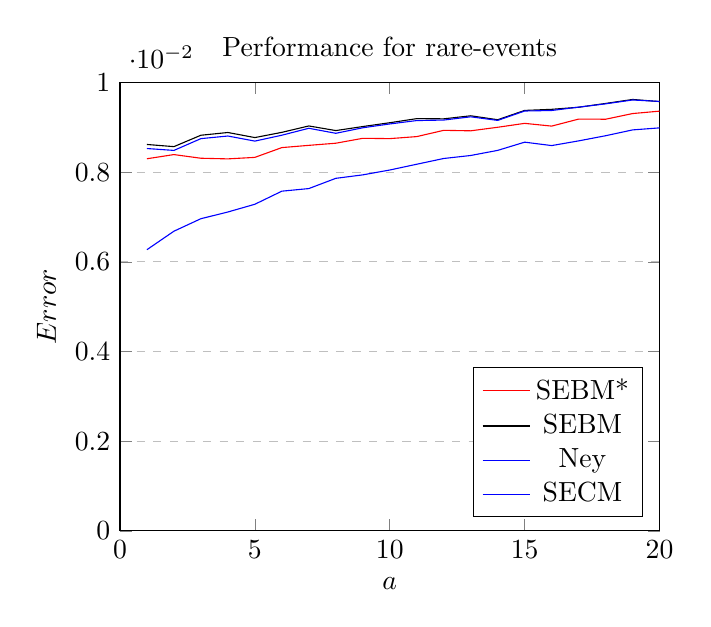
\begin{tikzpicture}[scale=1.0]
		\begin{axis}[
			title={Performance for rare-events},
			xlabel={$a$},
			xmin=0, xmax=20,
			ymin=0.000, ymax=0.01,
			ymajorgrids=true,
			ylabel={$Error$},
			grid style=dashed,
			xticklabel style={/pgf/number format/fixed},
			legend pos=south east,
		]
		\addplot[color=red] coordinates {
		(1,0.00829898628225)(2,0.00839191742155)(3,0.00831034375718)(4,0.00829616185199)(5,0.00832950631521)(6,0.00854788207454)(7,0.00859788647386)(8,0.00864539507562)(9,0.00875494343606)(10,0.00874804130022)(11,0.00879320206649)(12,0.00893286726698)(13,0.00892212687259)(14,0.00900143434975)(15,0.00908826041694)(16,0.00902723165099)(17,0.00918368988491)(18,0.00918072508884)(19,0.00930705761444)(20,0.00936085652527)
		};
\addlegendentry{SEBM*}
		\addplot[] coordinates {
		(1,0.00861758612646)(2,0.00856931333511)(3,0.00882336193996)(4,0.00888456557868)(5,0.00877127203762)(6,0.00888791399471)(7,0.00903070521197)(8,0.00892750294613)(9,0.00901735865911)(10,0.00910237180572)(11,0.00919387192857)(12,0.00918944397918)(13,0.00925732316038)(14,0.00916931563909)(15,0.00937697513676)(16,0.00940154091917)(17,0.00944782712404)(18,0.00953263660509)(19,0.00962165024385)(20,0.00957429275453)
		};
\addlegendentry{SEBM}
		\addplot[color=blue] coordinates {
		(1,0.00627042393191)(2,0.00668283560602)(3,0.00696175803194)(4,0.00711122084588)(5,0.00728404764124)(6,0.00757582039795)(7,0.00763393965732)(8,0.00786227870242)(9,0.00793950292667)(10,0.00804775959656)(11,0.00817661699722)(12,0.00830499867171)(13,0.00837197170234)(14,0.00848570355671)(15,0.00866904091263)(16,0.00859262838231)(17,0.00869764757103)(18,0.00881244467649)(19,0.00894236872475)(20,0.00898769050537)
		};
\addlegendentry{Ney}
		\addplot[color=blue] coordinates {
		(1,0.00852711828901)(2,0.00848494072214)(3,0.00874773654002)(4,0.00880609825734)(5,0.00869268282241)(6,0.00882394889482)(7,0.00897875778344)(8,0.0088667004212)(9,0.0089897364589)(10,0.00907540185807)(11,0.00915081153869)(12,0.00916218423184)(13,0.0092344860602)(14,0.00915425878397)(15,0.00936396139817)(16,0.00937527442835)(17,0.00945006806042)(18,0.00952384116565)(19,0.0096100208579)(20,0.00957776196452)
		};
\addlegendentry{SECM}
		\end{axis}
	\end{tikzpicture}
    \caption{Average error of three stratified random sampling methods for the uniform-Bernoulli data sets of Section~\ref{sec:dataset2}, plotted against success parameter $a$, across 20,000 rounds.}
	\label{biggraph3}
\end{figure}

